\documentclass[twocolumn]{article}

\usepackage{amsmath}
\usepackage{caption}
\usepackage{graphicx}
\usepackage{float}
\usepackage{subcaption}

% Make table names in captions boldfaced
\captionsetup[table]{labelfont=bf}
\captionsetup[figure]{labelfont=bf}

%opening
\title{Measuring the Zeeman Effect}
\author{}

\begin{document}

\maketitle

\begin{abstract}
	
\end{abstract}

\section{Introduction} \label{sec:Intro}
	\subsection{Historical Background}

	\subsection{Theory of the Zeeman Effect} \label{sec:Theory}
		
\section{Methods and Procedures}
	To study the Zeeman effect, observations of a mercury lamp were made first with no magnetic field and $90\deg$ polarization, then with an approximately $1T$ magnetic field.
	Observations with a magnetic field included:
	\begin{itemize}
		\item $90\deg$ (field-perpendicular) polarization
		\item $0\deg$ (field-parallel) polarization 
		\item No polarization
		\item Axial B-field at polarization varying from $90\deg$ to $0\deg$
	\end{itemize}
	
	\begin{figure*}[t]
		\centering
		\begin{subfigure}{0.55\textwidth}
			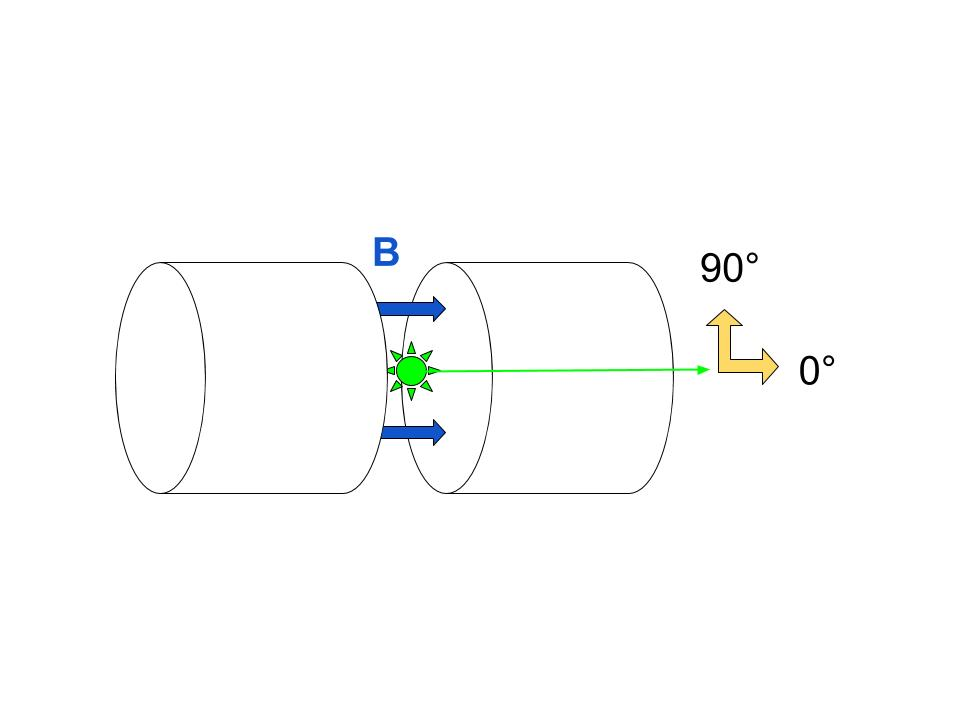
\includegraphics[width = 0.8\textwidth]{Images/FieldConfigA.jpg}
			\caption{\textbf{Perpendicular field configuration.}}
			\label{subfig:PerpFieldConfig}
		\end{subfigure}%
		\begin{subfigure}{0.55\textwidth}
			\centering
			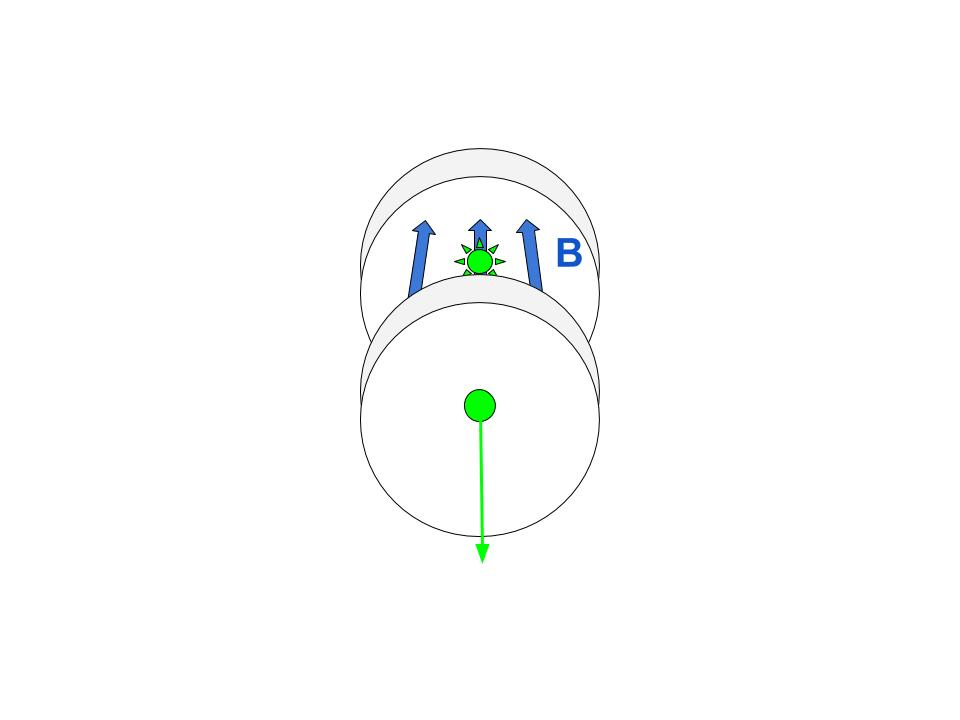
\includegraphics[width=0.8\textwidth]{Images/FieldConfigB.jpg}
			\caption{\textbf{Axial field configuration.}}
			\label{subfig:AxialFieldConfig}
		\end{subfigure}%
		\caption{\textbf{The two magnetic field configurations observed. In (\ref{subfig:PerpFieldConfig}), the magnetic field is oriented perpendicularly to the path of the observed light from the mercury lamp. In configuration (\ref{subfig:AxialFieldConfig}), light from the lamp travels along the magnetic field lines down the center of one of the solenoids through a sight hole.}}
		\label{fig:FieldConfig}
	\end{figure*}
	
	\subsection{Method Description} \label{subsec:MethodDescription}
	
\section{Data and Results} \label{sec:DataAndResults}
 
	\subsection{Spectra Through a Perpendicular Magnetic Field}
		\subsubsection{Spectra with Field-Perpendicular Polarization}
	
		\subsubsection{Spectra with Field-Parallel Polarization}
	
	\subsection{Spectra Along an Axial Magnetic Field}
	
	\subsection{Measurement of the Bohr Magneton} \label{subsec:BohrMagneton}
		With the precise measurement of spectral line splitting in the presence of the perpendicular magnetic field, it was possible to measure the value of the Bohr magneton.
	

\section{Conclusion} \label{sec:Conclusion}

\end{document}
